
% \renewcommand{\thefigure}{A.\arabic{section}.\arabic{figure}hhh}
\counterwithin{figure}{section}
\setcounter{section}{4} % Assuming section A.4 corresponds to section 4
\setcounter{figure}{0}  % Reset figure counter for this section

% Set caption justification to justified
\captionsetup{justification=justified}
\captionsetup{skip=15pt}

%%%%%%%%%%%%%%%%%%%%
%%% MAIN FIGURES %%%
%%%%%%%%%%%%%%%%%%%%

%%%%%%%%%%%%%%%%%%%%
%% SUPPLEMENTARY %%%
%%%%%%%%%%%%%%%%%%%%

\begin{figure}[htbp]
  \centering
  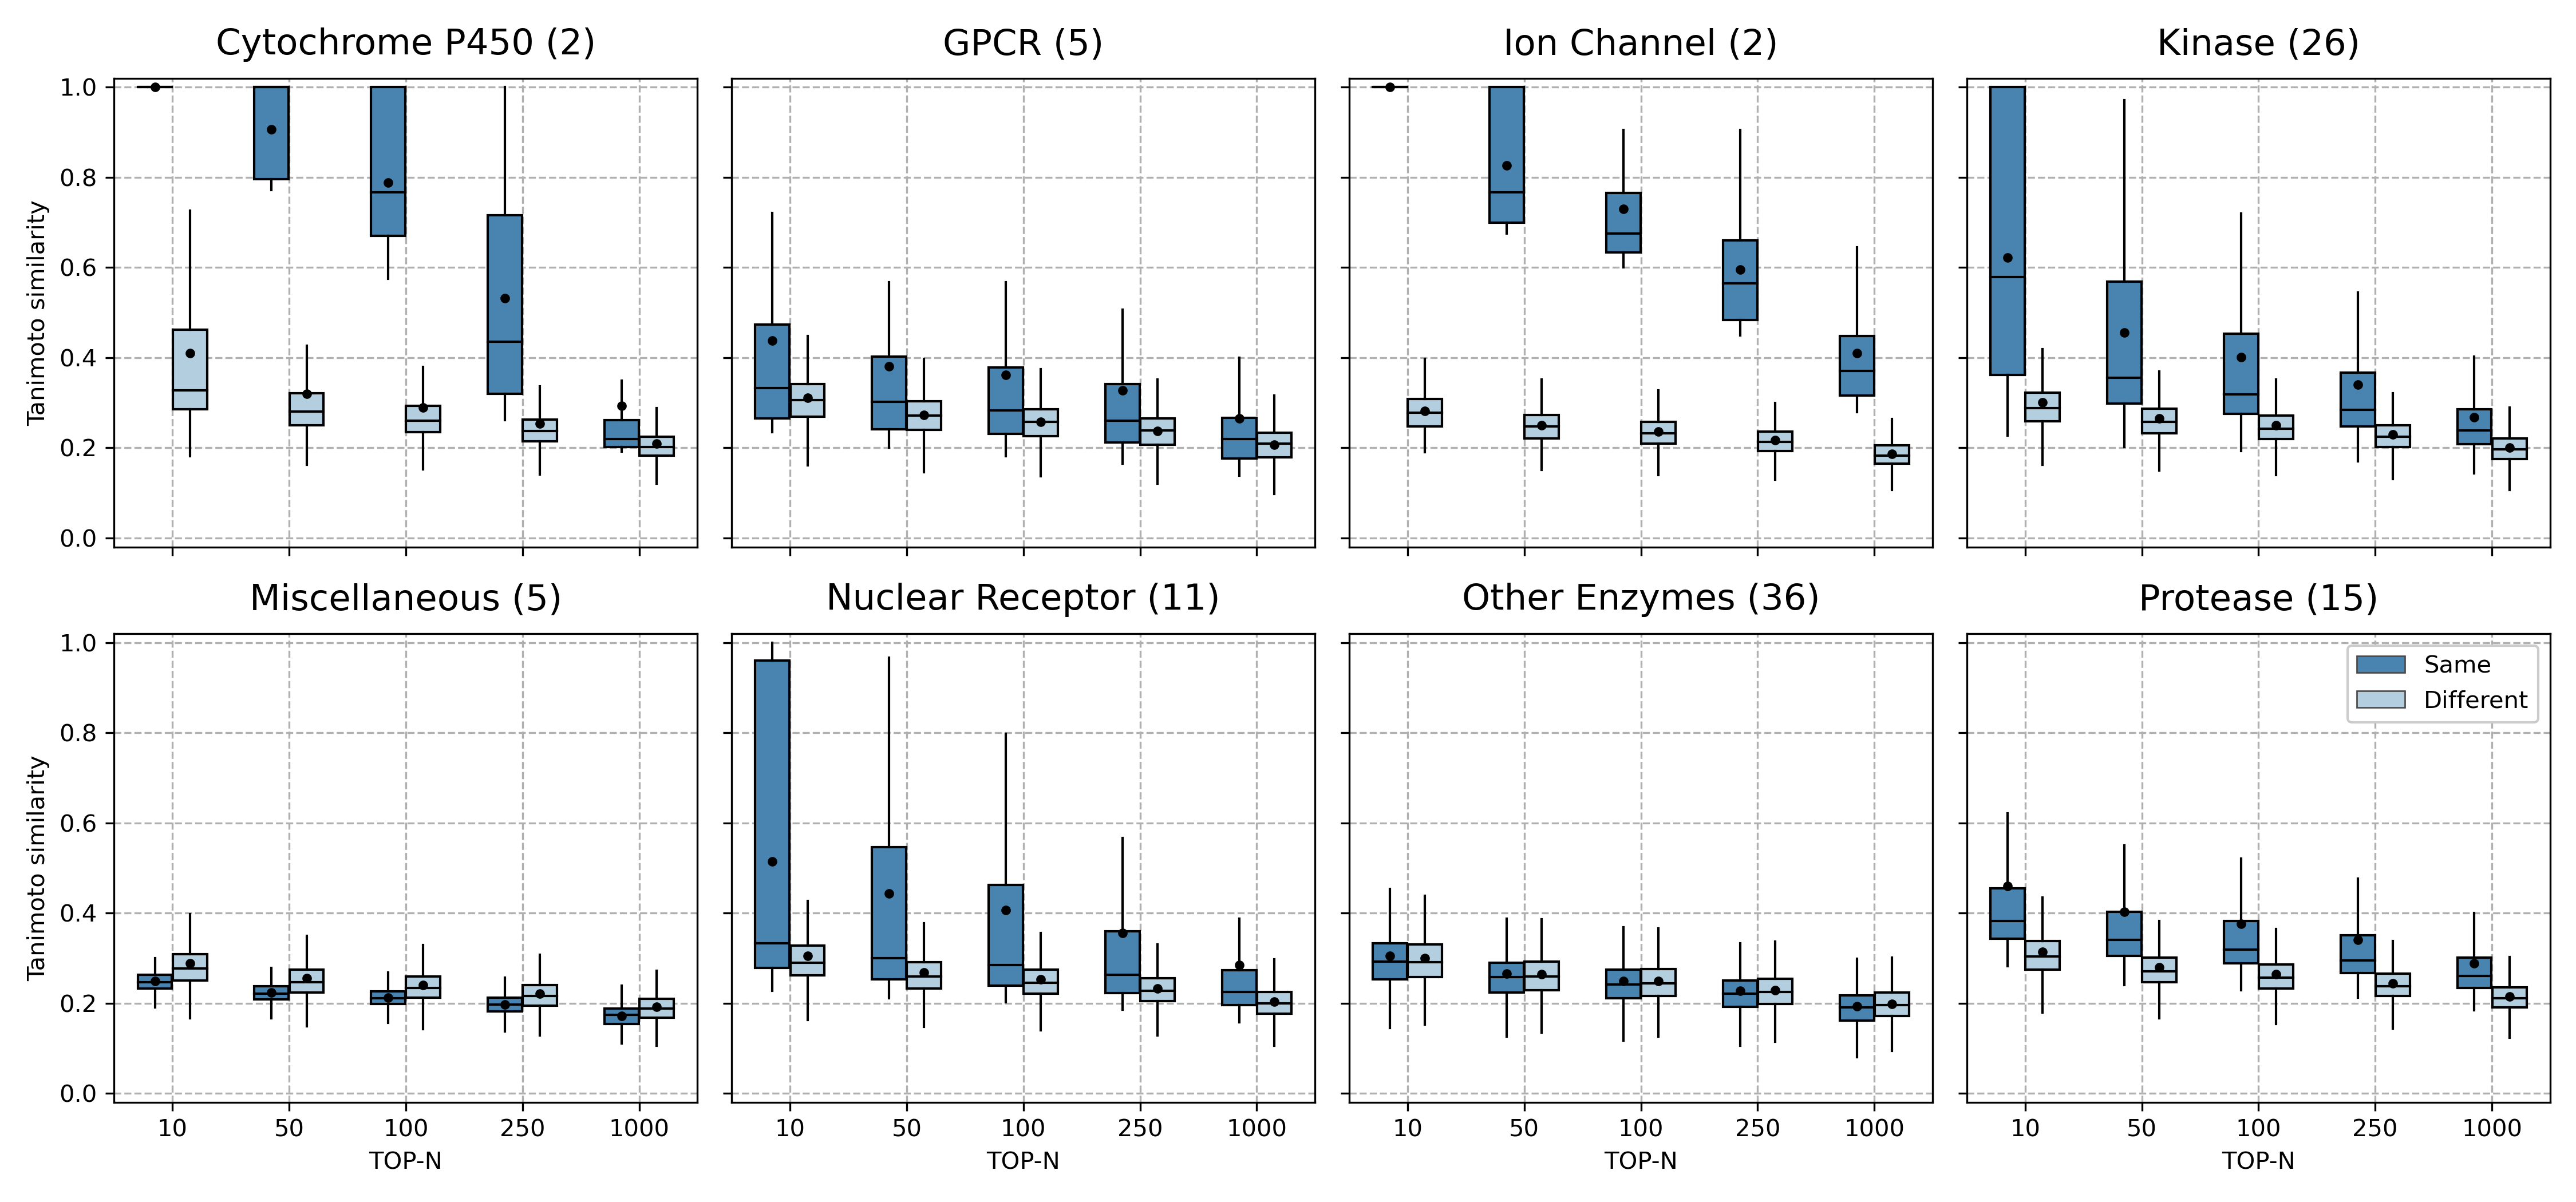
\includegraphics[width=\linewidth]{figures/PocketVec/Supplementary/FigS1.png}
  \caption{Similar proteins bind similar active compounds. For each protein family (e.g. Cytochrome P450, GPCR, etc.) we compared all active compounds between protein pairs from the same family (Same) and from different families (Different). Compounds were compared on the basis of their Tanimoto Similarities (y-axis, ECFP4 with 2048 bits using RDKit – https://rdkit.org) and only the TOP-N (x-axis: 10, 50, 100, 250, 1000) highest similarities were considered per each family. All distributions of Same and Different categories are significantly different (Mann-Whitney U test, pvalue <0.05, alternative greater using SciPy\cite{virtanen_scipy_2020}) except Miscellaneous (10, 50, 100, 250, 1000) and Other Enzymes (10, 50, 100, 250, 1000). Box plots indicate median (middle line), 25th, 75th percentile (box), and max and min value within the 1.5*25th and 1.5*75th percentile range (whiskers). Black dots represent mean values. The number of proteins within each family is specified in the title in parenthesis. Data was downloaded from \href{http://dude.docking.org}{http://dude.docking.org} in January 2023.}
  \label{FigS1}
\end{figure}


\begin{figure}[htbp]
  \centering
  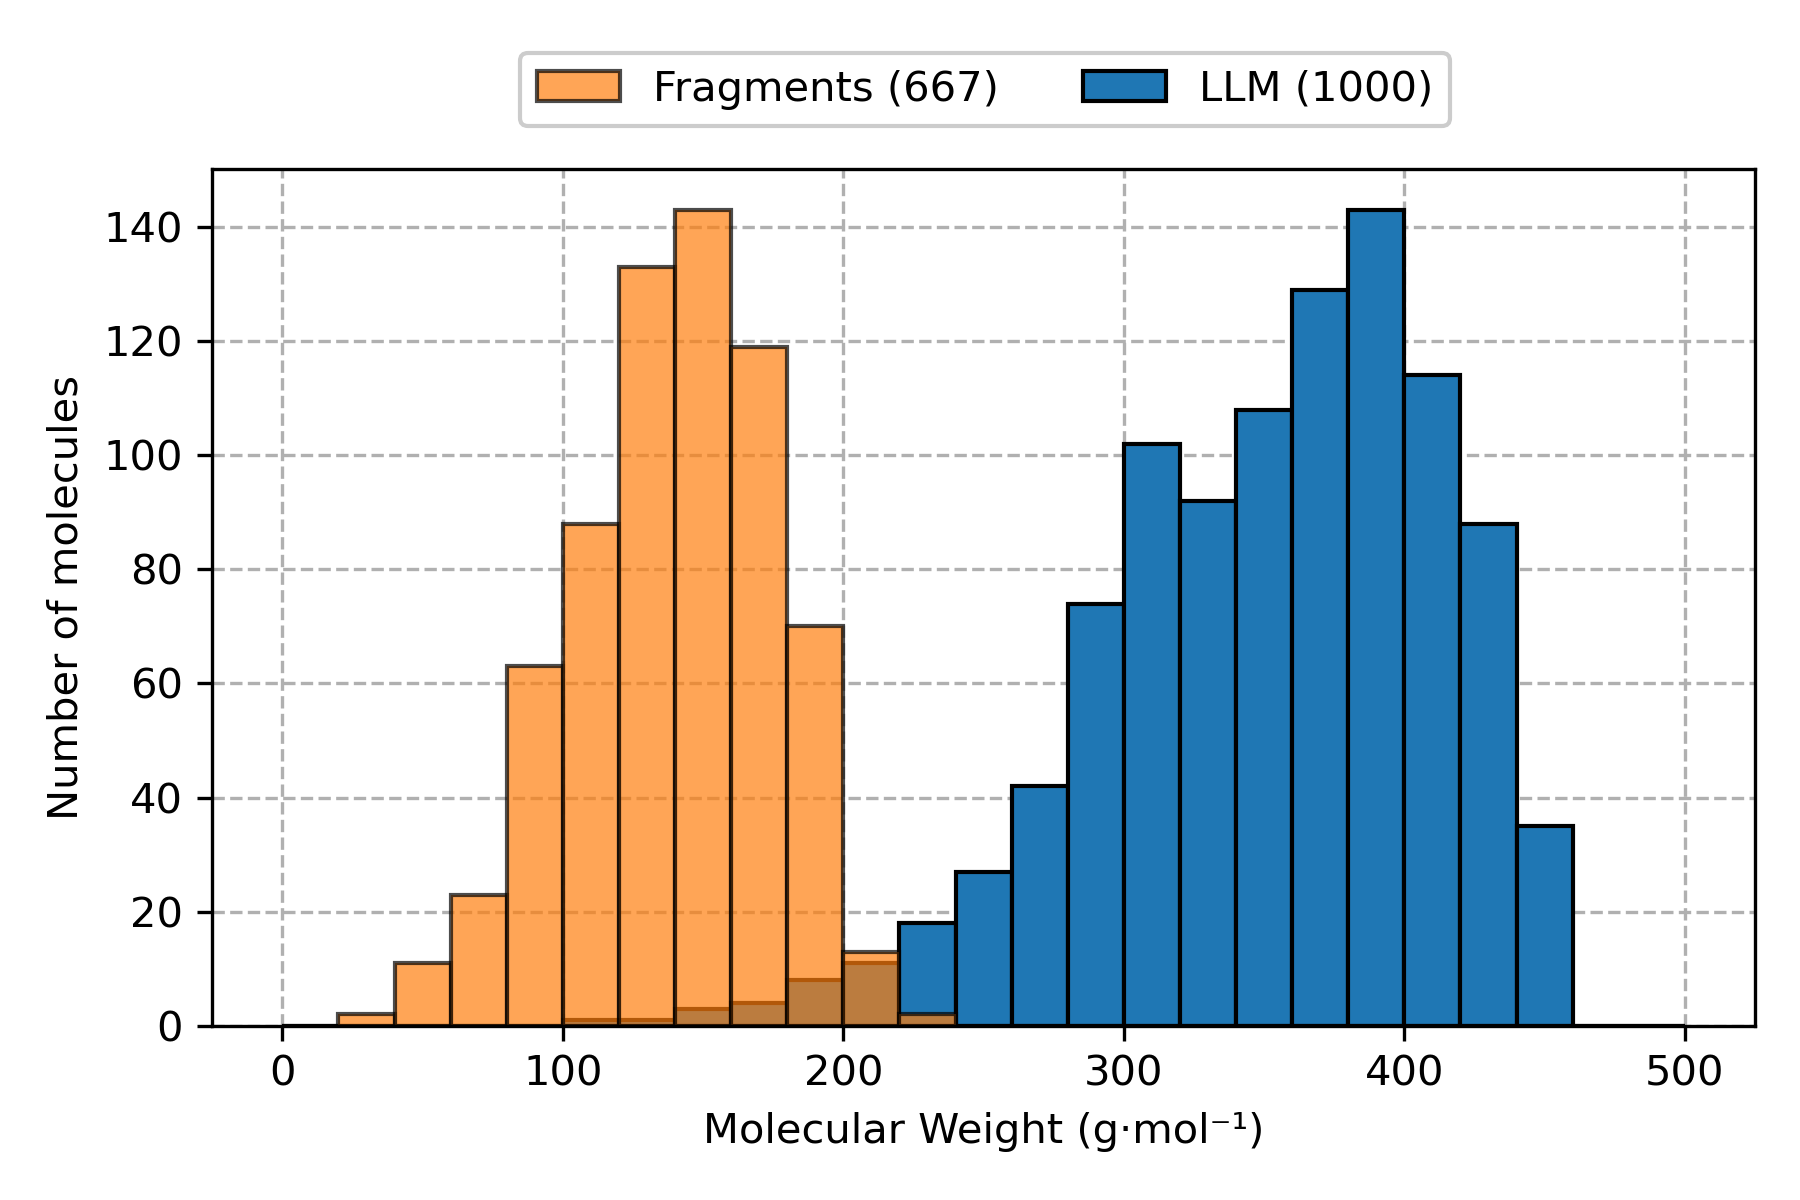
\includegraphics[width=0.65\linewidth]{figures/PocketVec/Supplementary/FigS2.png}
  \caption{
  Histograms of molecular weights (x-axis) from fragments (667, orange) and lead-like molecules (1,000, blue).
  }
  \label{FigS2}
\end{figure}


\begin{figure}[htbp]
  \centering
  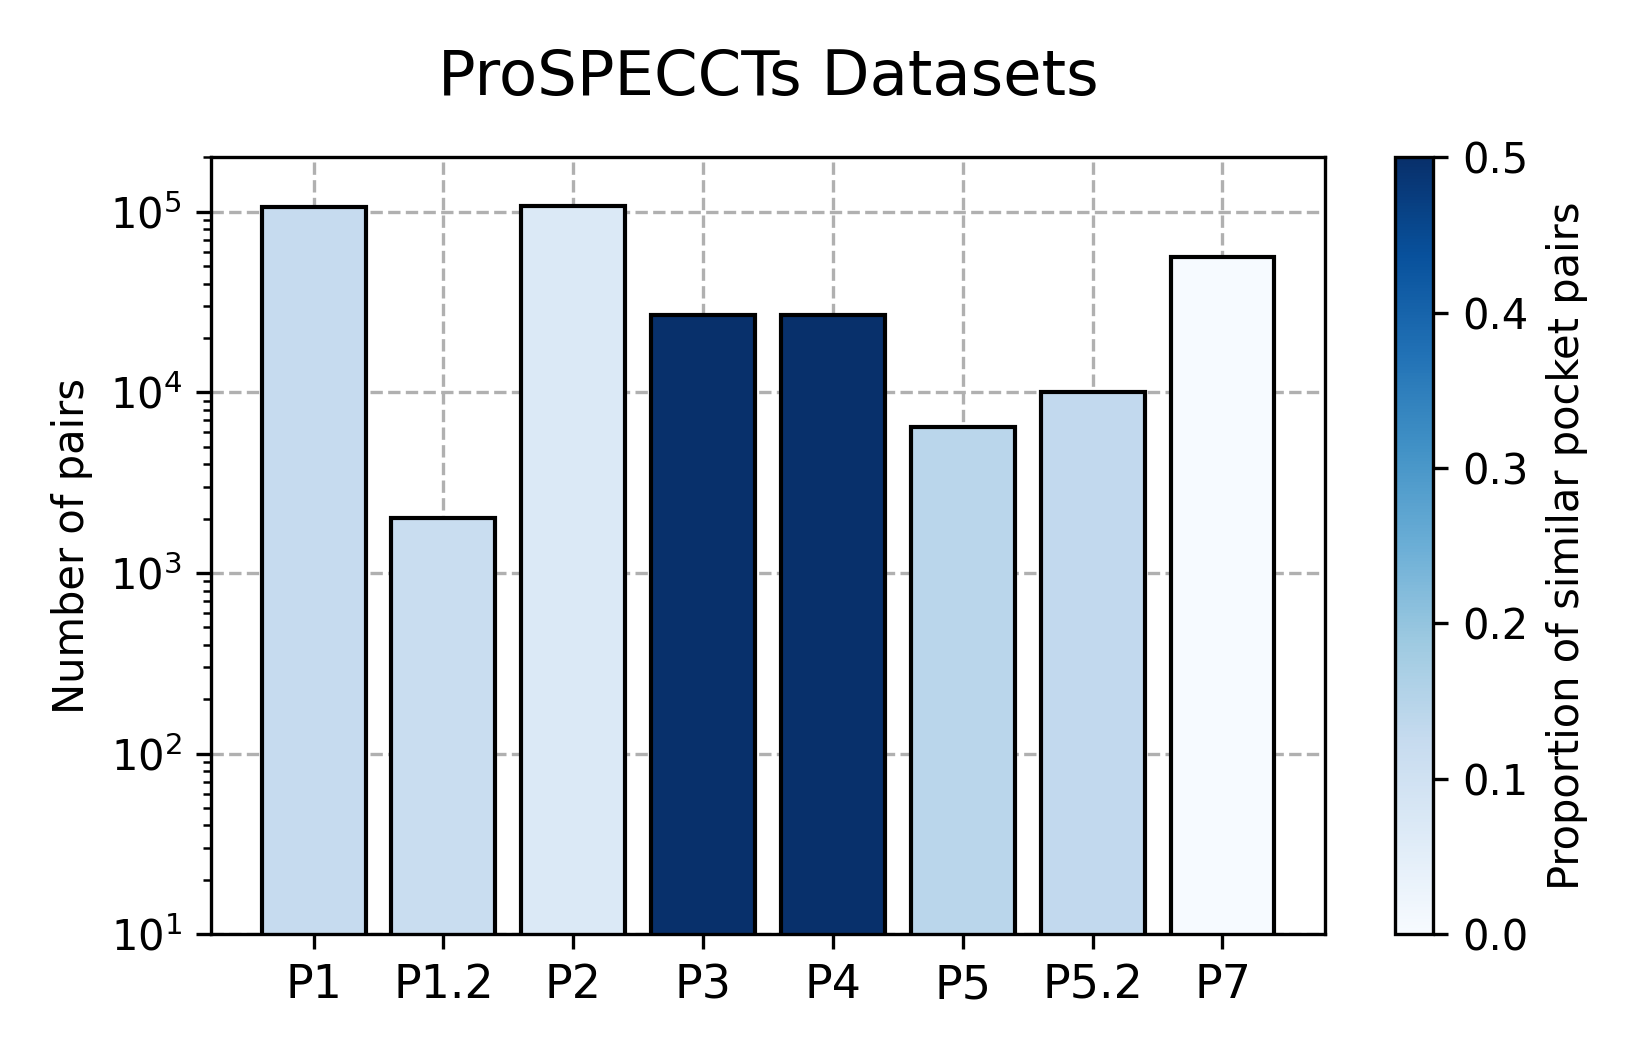
\includegraphics[width=0.75\linewidth]{figures/PocketVec/Supplementary/FigS3.png}
  \caption{
  ProSPECCTs overview. Each bar represents a ProSPECCT dataset (x-axis) and indicates the number of protein-ligand binding site pairs (y-axis) together with the proportion of similar pocket pairs within each dataset (color tone). Please, see the Online Methods section for a detailed description of each dataset.
  }
  \label{FigS3}
\end{figure}


\begin{figure}[htbp]
  \centering
  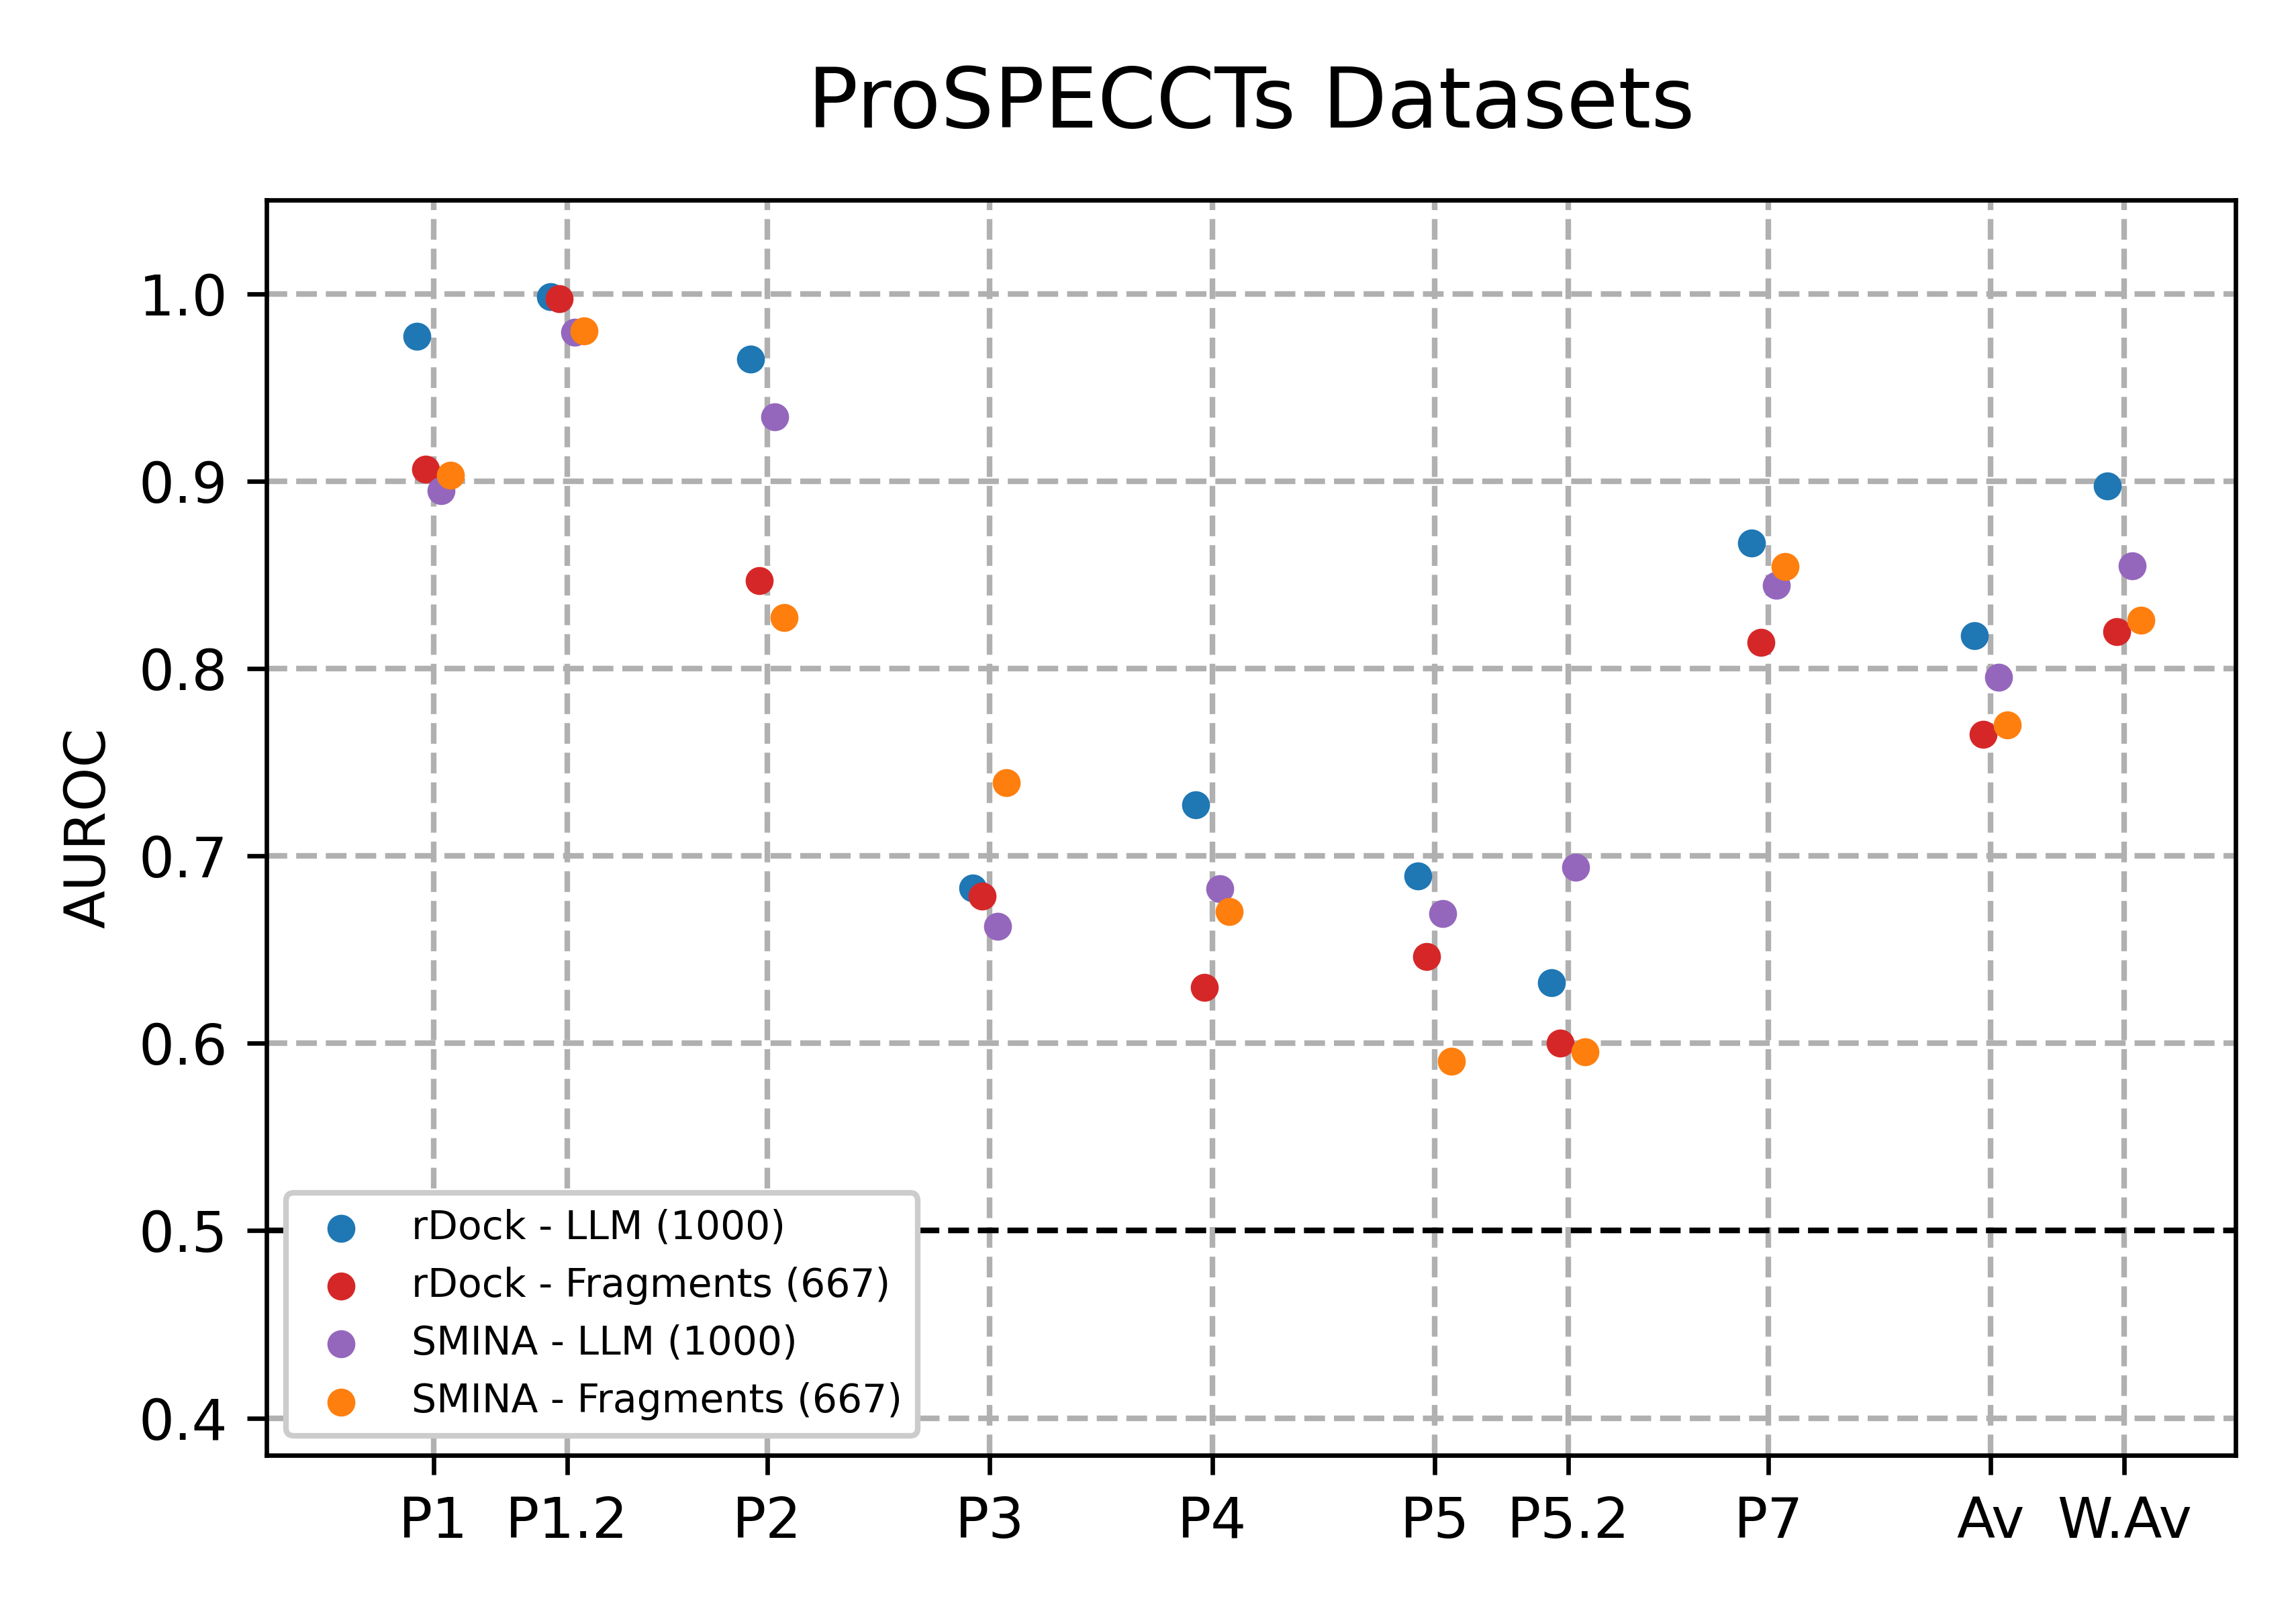
\includegraphics[width=0.65\linewidth]{figures/PocketVec/Supplementary/FigS4.png}
  \caption{
  Performances (AUROC, y-axis) among ProSPECCTs datasets (x-axis). Each colored dot represents the individual performance of our strategies with all possible combinations of docking approaches (rDock and SMINA) and compound collections (1,000 LLM and 667 fragments). Av. values represent the average performance among ProSPECCTs datasets for each individual strategy and W. Av. values weight the average value according to the number of pairs within each dataset.
  }
  \label{FigS4}
\end{figure}


\begin{figure}[htbp]
  \centering
  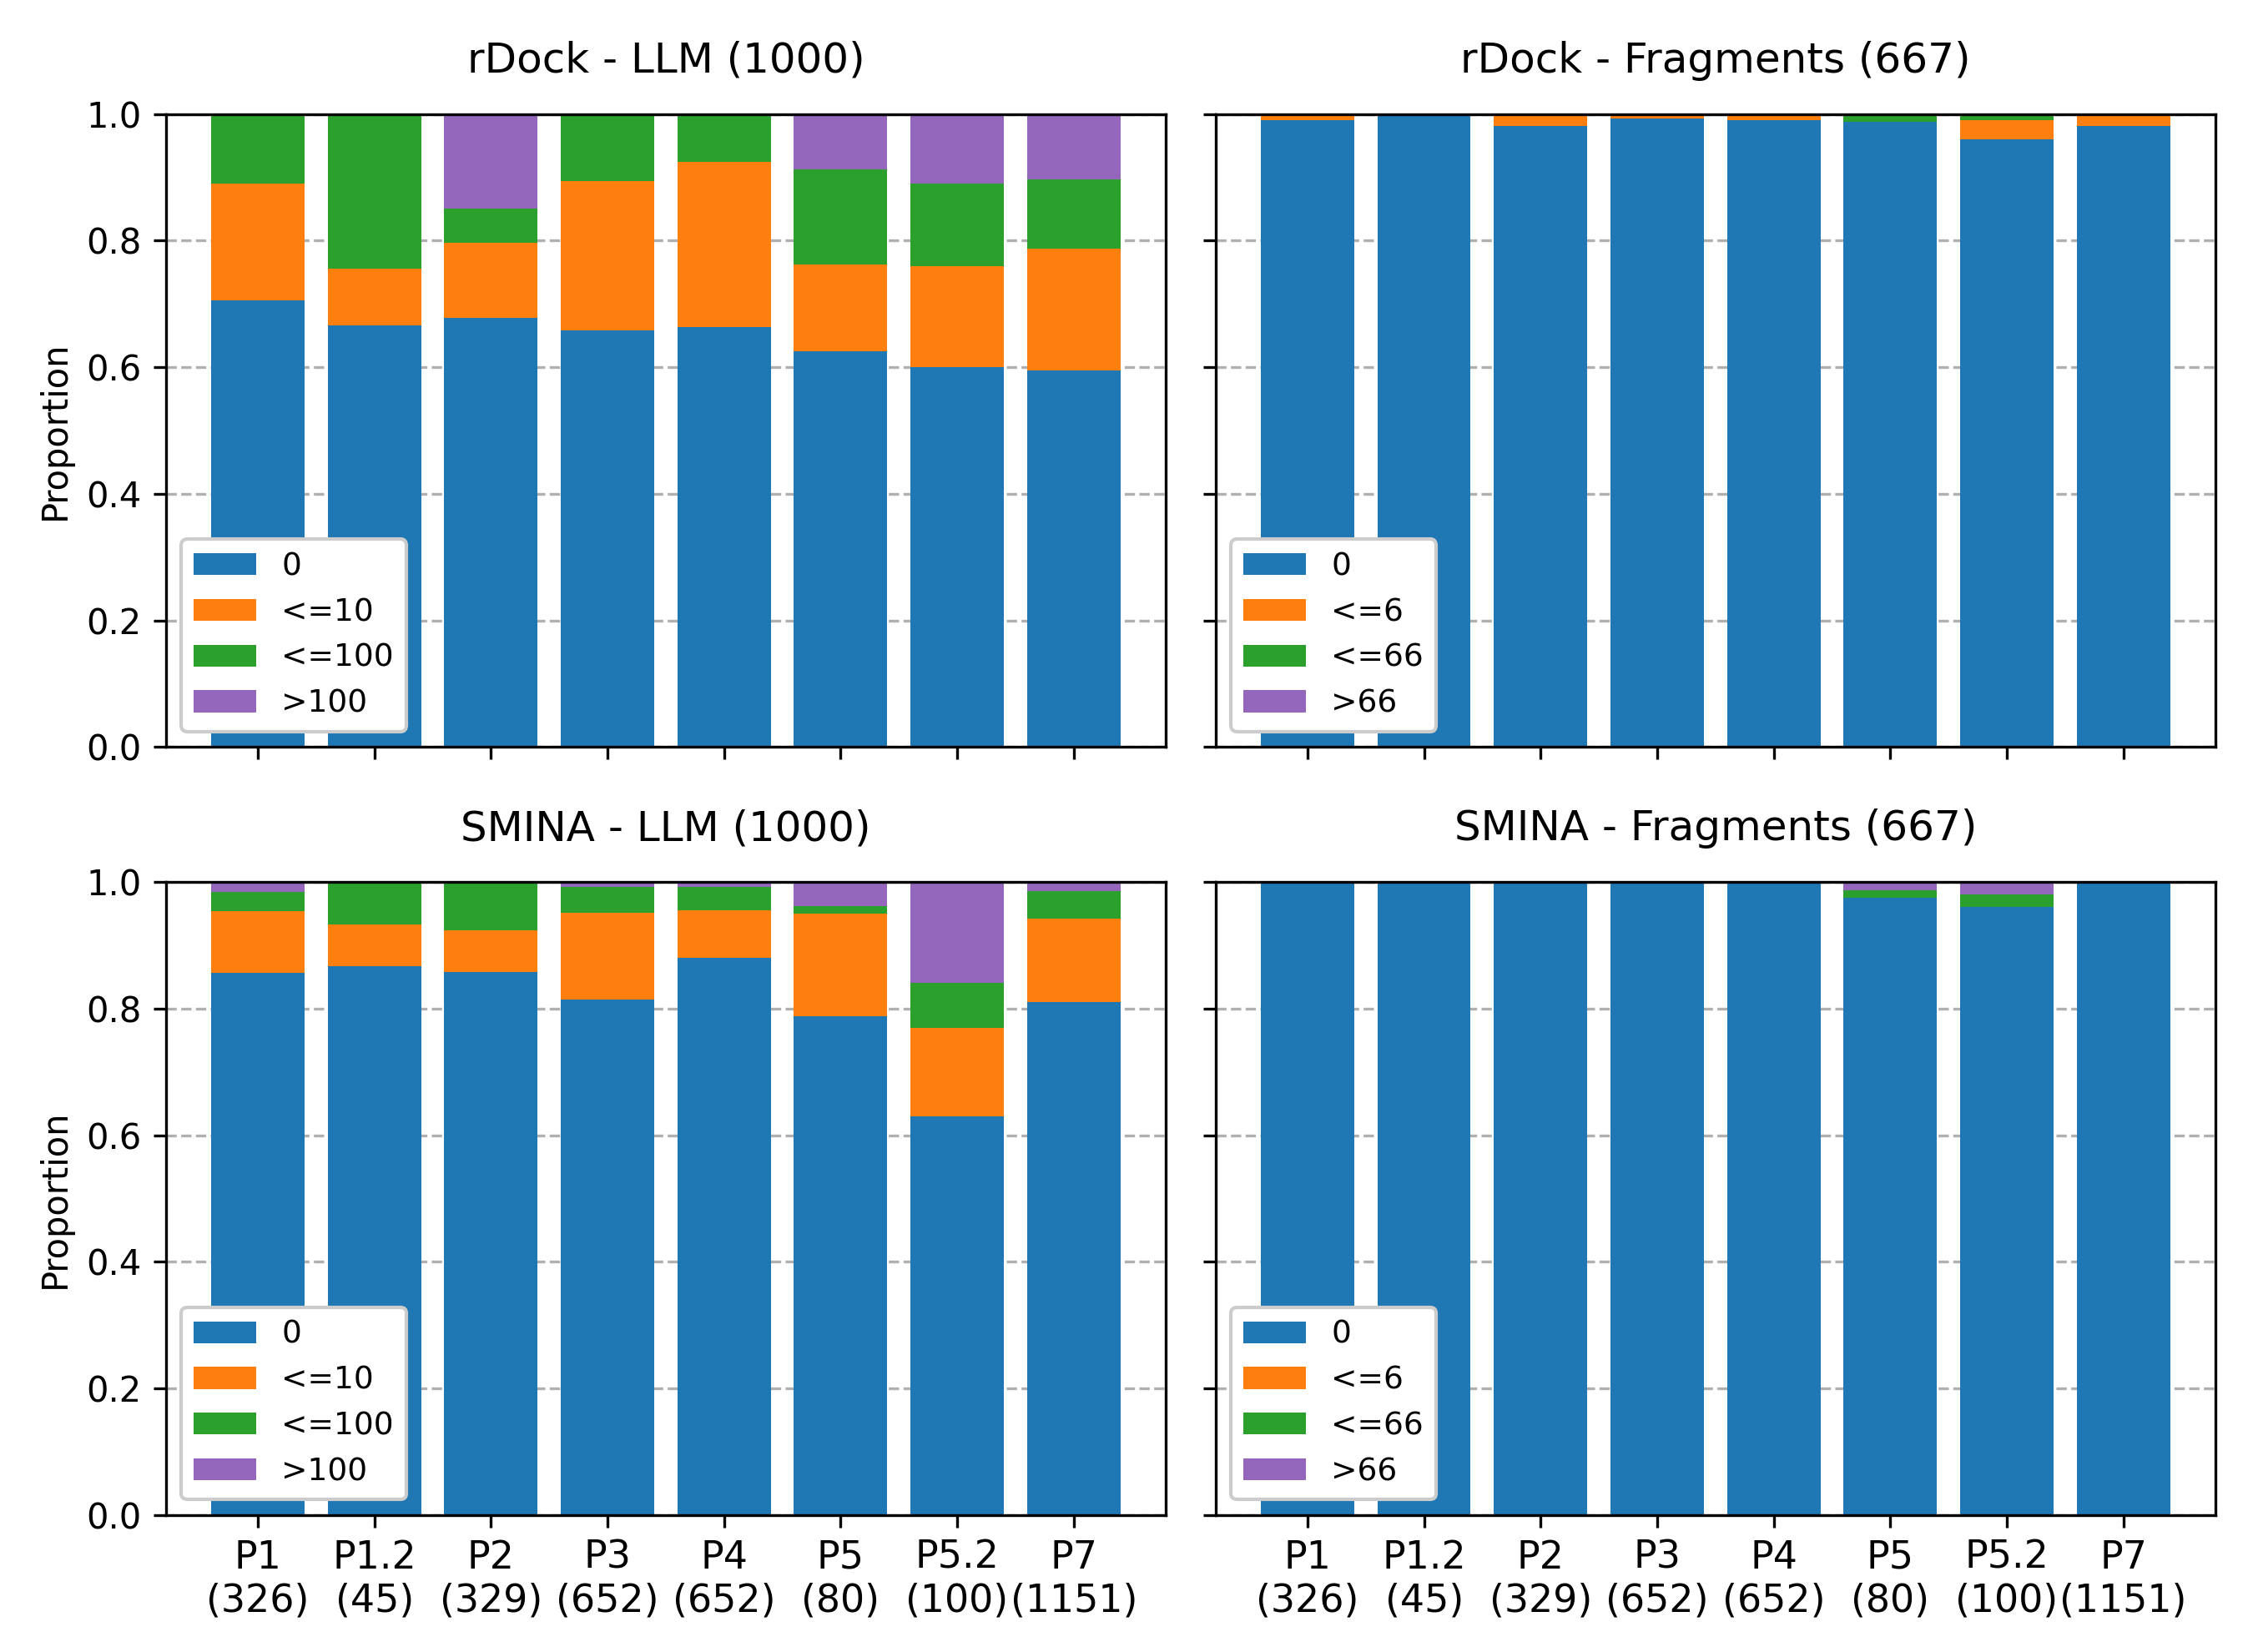
\includegraphics[width=0.75\linewidth]{figures/PocketVec/Supplementary/FigS5.png}
  \caption{
  Proportion of outlier molecules. Colored bars represent the proportion of outlier molecules (y-axis) within each ProSPECCTs dataset (x-axis) for each combination of docking method (rDock and SMINA) and compound collection (1,000 LLM and 667 fragments). Colors indicate the number of outlier molecules assigned to each structure. The number of structures per dataset is specified in parenthesis (x labels).
  }
  \label{FigS5}
\end{figure}

\begin{figure}[htbp]
  \centering
  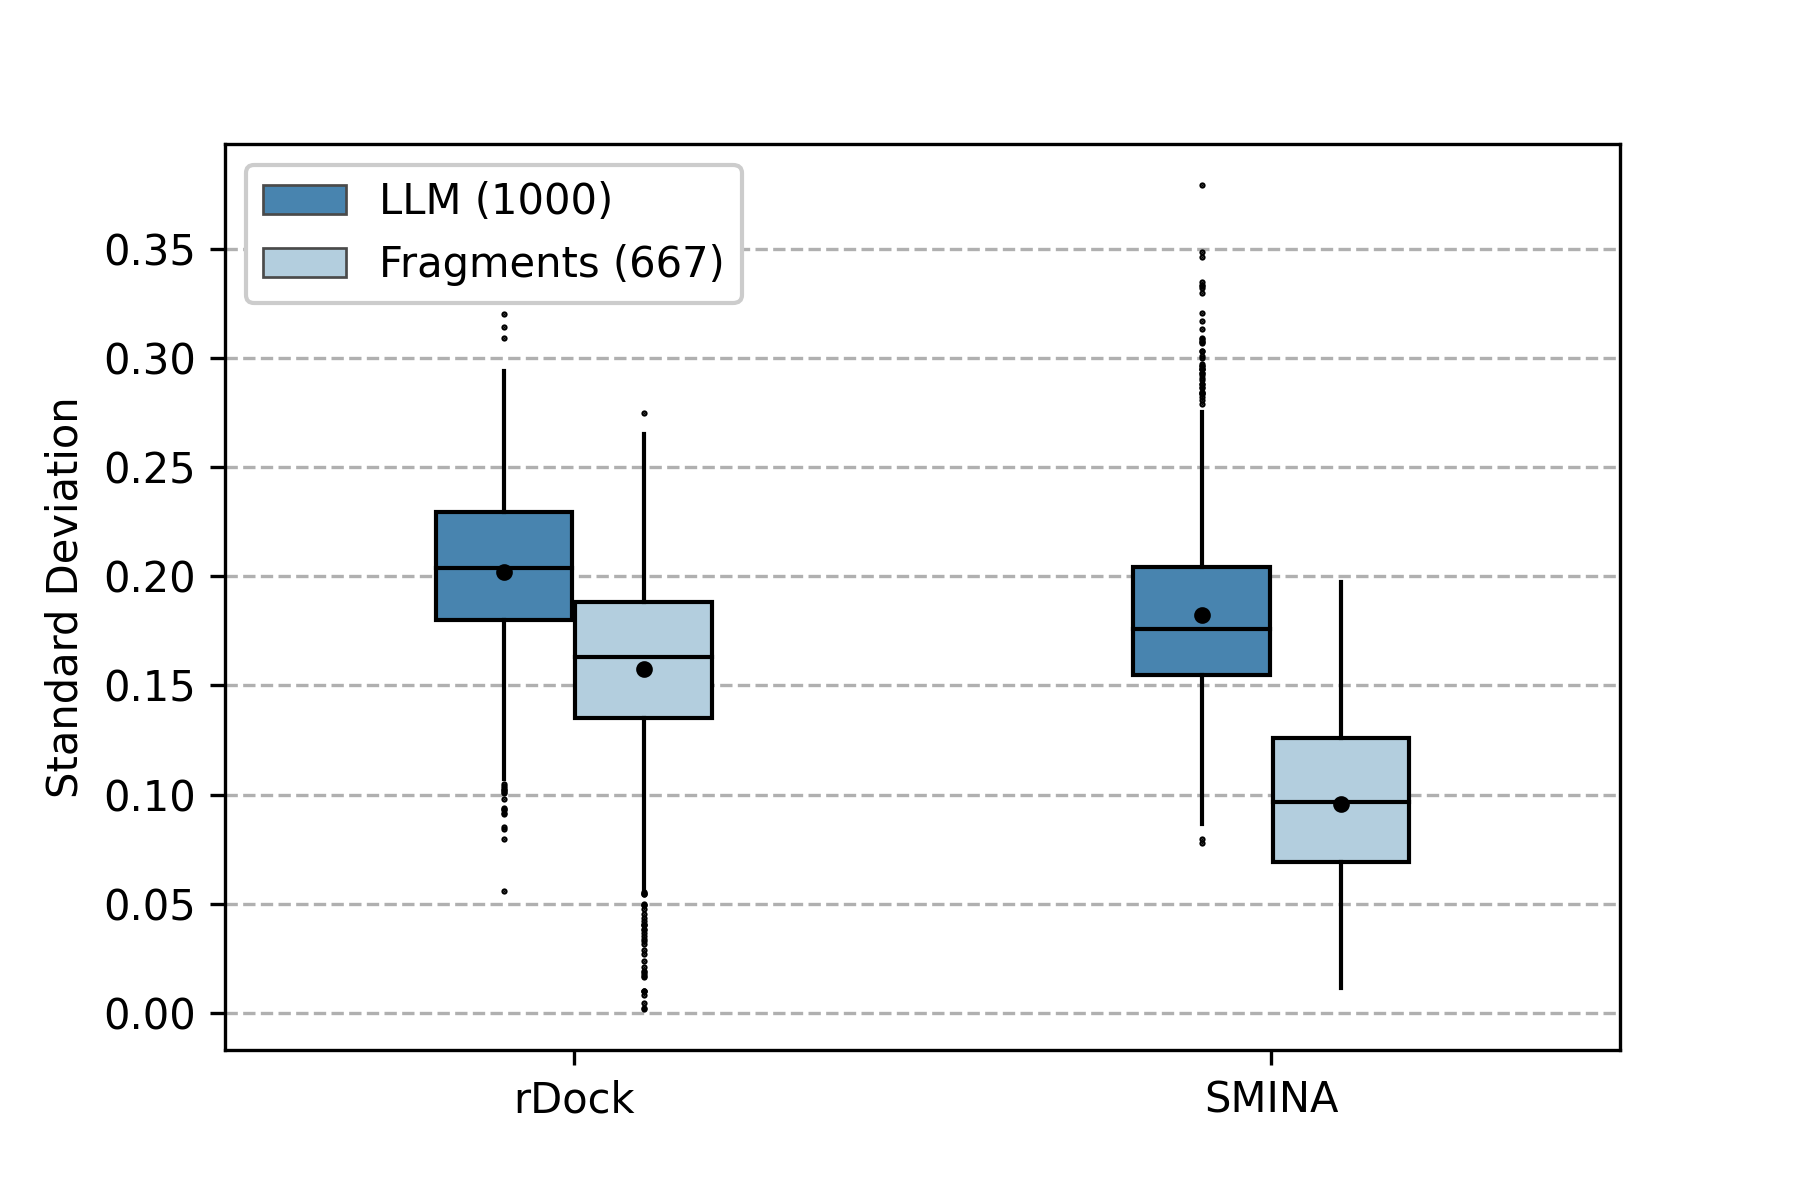
\includegraphics[width=0.55\linewidth]{figures/PocketVec/Supplementary/FigS6.png}
  \caption{
  Ranking diversity differences. For each docking method (rDock and SMINA) and compound collection (1,000 LLM and 667 fragments) ProSPECCTs pockets were considered all at once (3,335 pockets) and the standard deviation (in terms of rankings) was calculated for each tested compound. For both docking strategies standard deviation distributions between LLM and fragments are statistically different (Mann-Whitney U test, p<10-70 in both cases). Box plots indicate median (middle line), 25th, 75th percentile (box), and max and min value within the 1.5*25th and 1.5*75th percentile range (whiskers). Black dots represent mean values.
  }
  \label{FigS6}
\end{figure}


\begin{figure}[htbp]
  \centering
  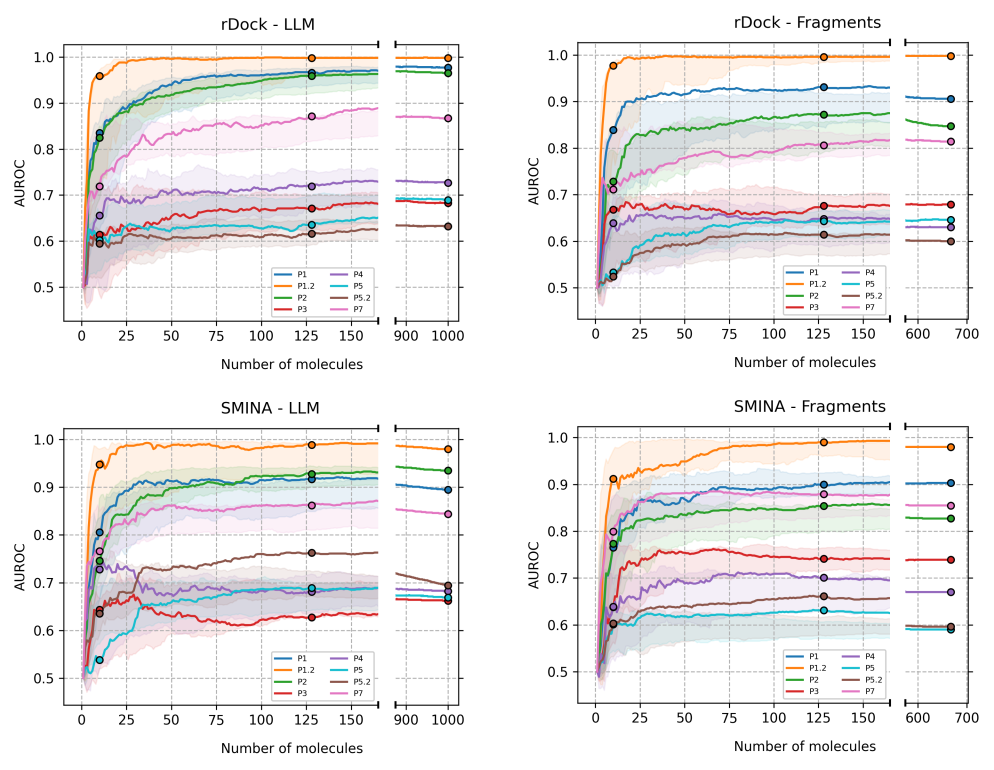
\includegraphics[width=1\linewidth]{figures/PocketVec/Supplementary/FigS7.png}
  \caption{
  Performances (AUROC, y-axis) of our descriptors among ProSPECCTs datasets (color, P6 and P6.2 not included. For further details, please see Online Methods) generated with a varying number of predefined compounds (x-axis, from 1 to complete sets, sorted by entropy). Colored points indicate the performance at 10, 128 and 1,000/667 molecules. Colored areas represent the best and worst performances obtained with randomly (x100) selected compounds (not sorted by entropy values). Each subplot corresponds to a combination of docking method (rDock and SMINA) and compound collection (1,000 LLM and 667 fragments).   
  }
  \label{FigS7}
\end{figure}

\begin{figure}[htbp]
  \centering
  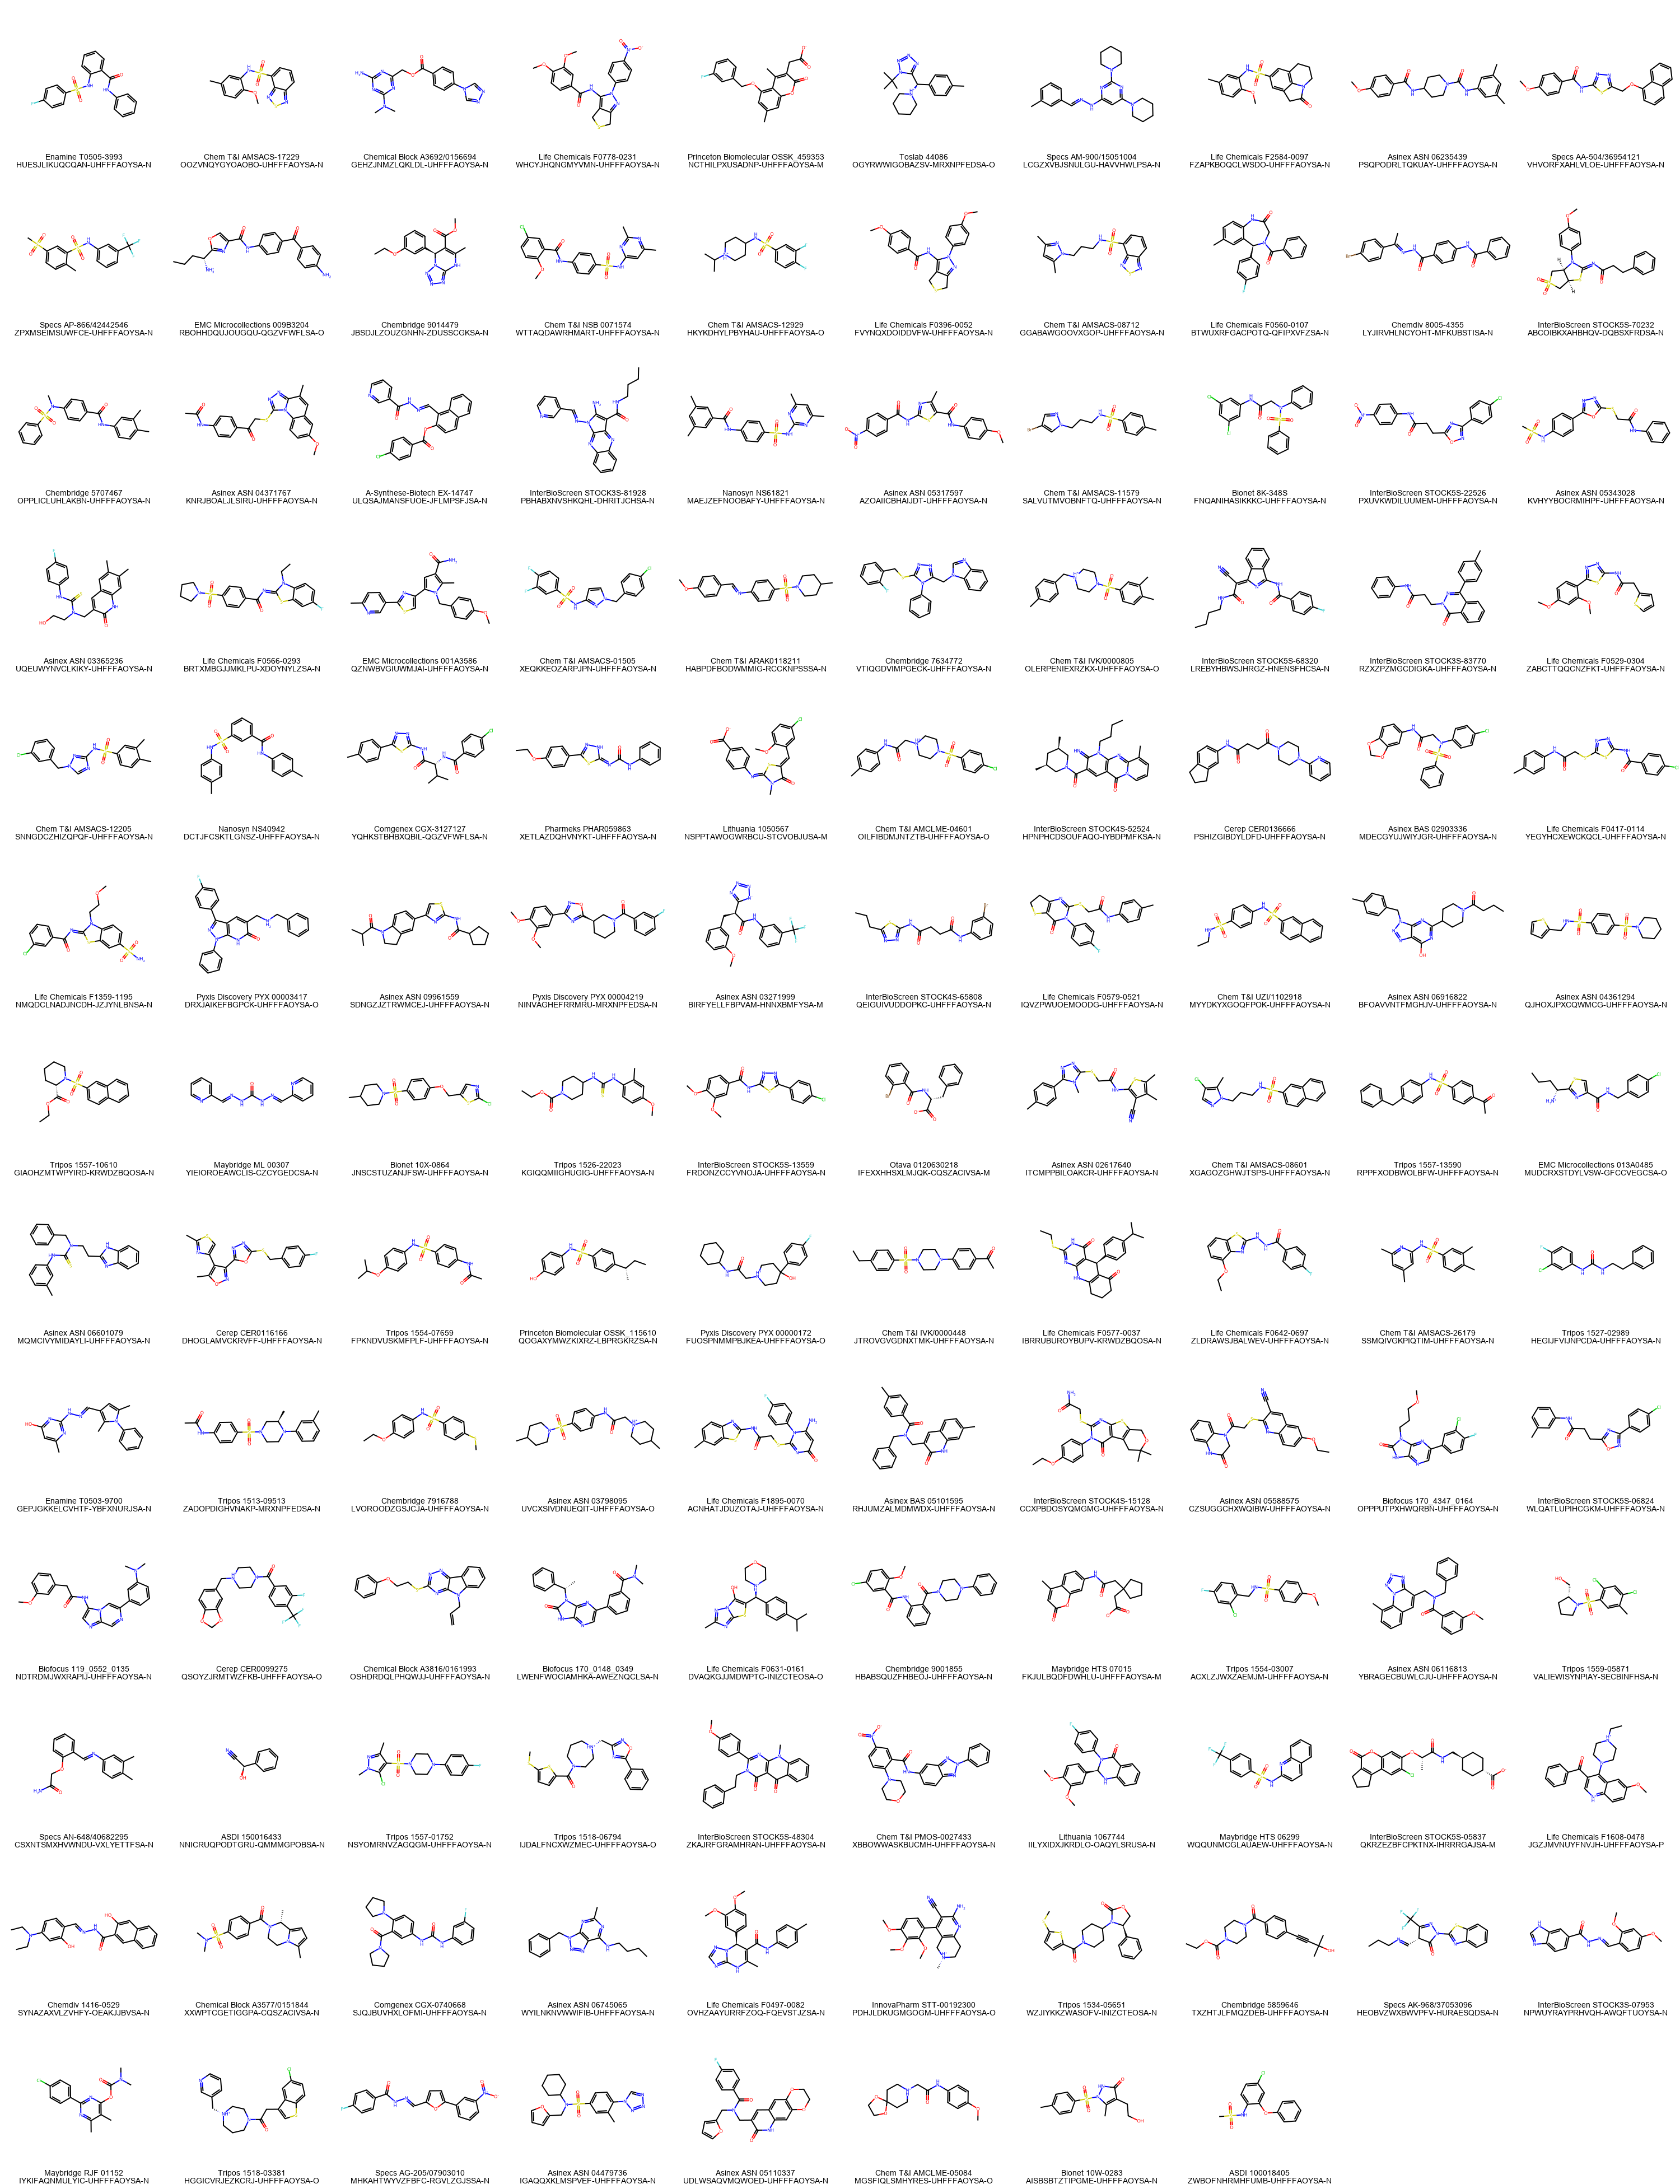
\includegraphics[width=0.9\linewidth]{figures/PocketVec/Supplementary/FigS8_v2.png}
  \caption{
  Standard 128 lead-like molecules used to generate PocketVec descriptors, including their commercial names and InChiKeys.
  }
  \label{FigS8_v2}
\end{figure}

\begin{figure}[htbp]
  \centering
  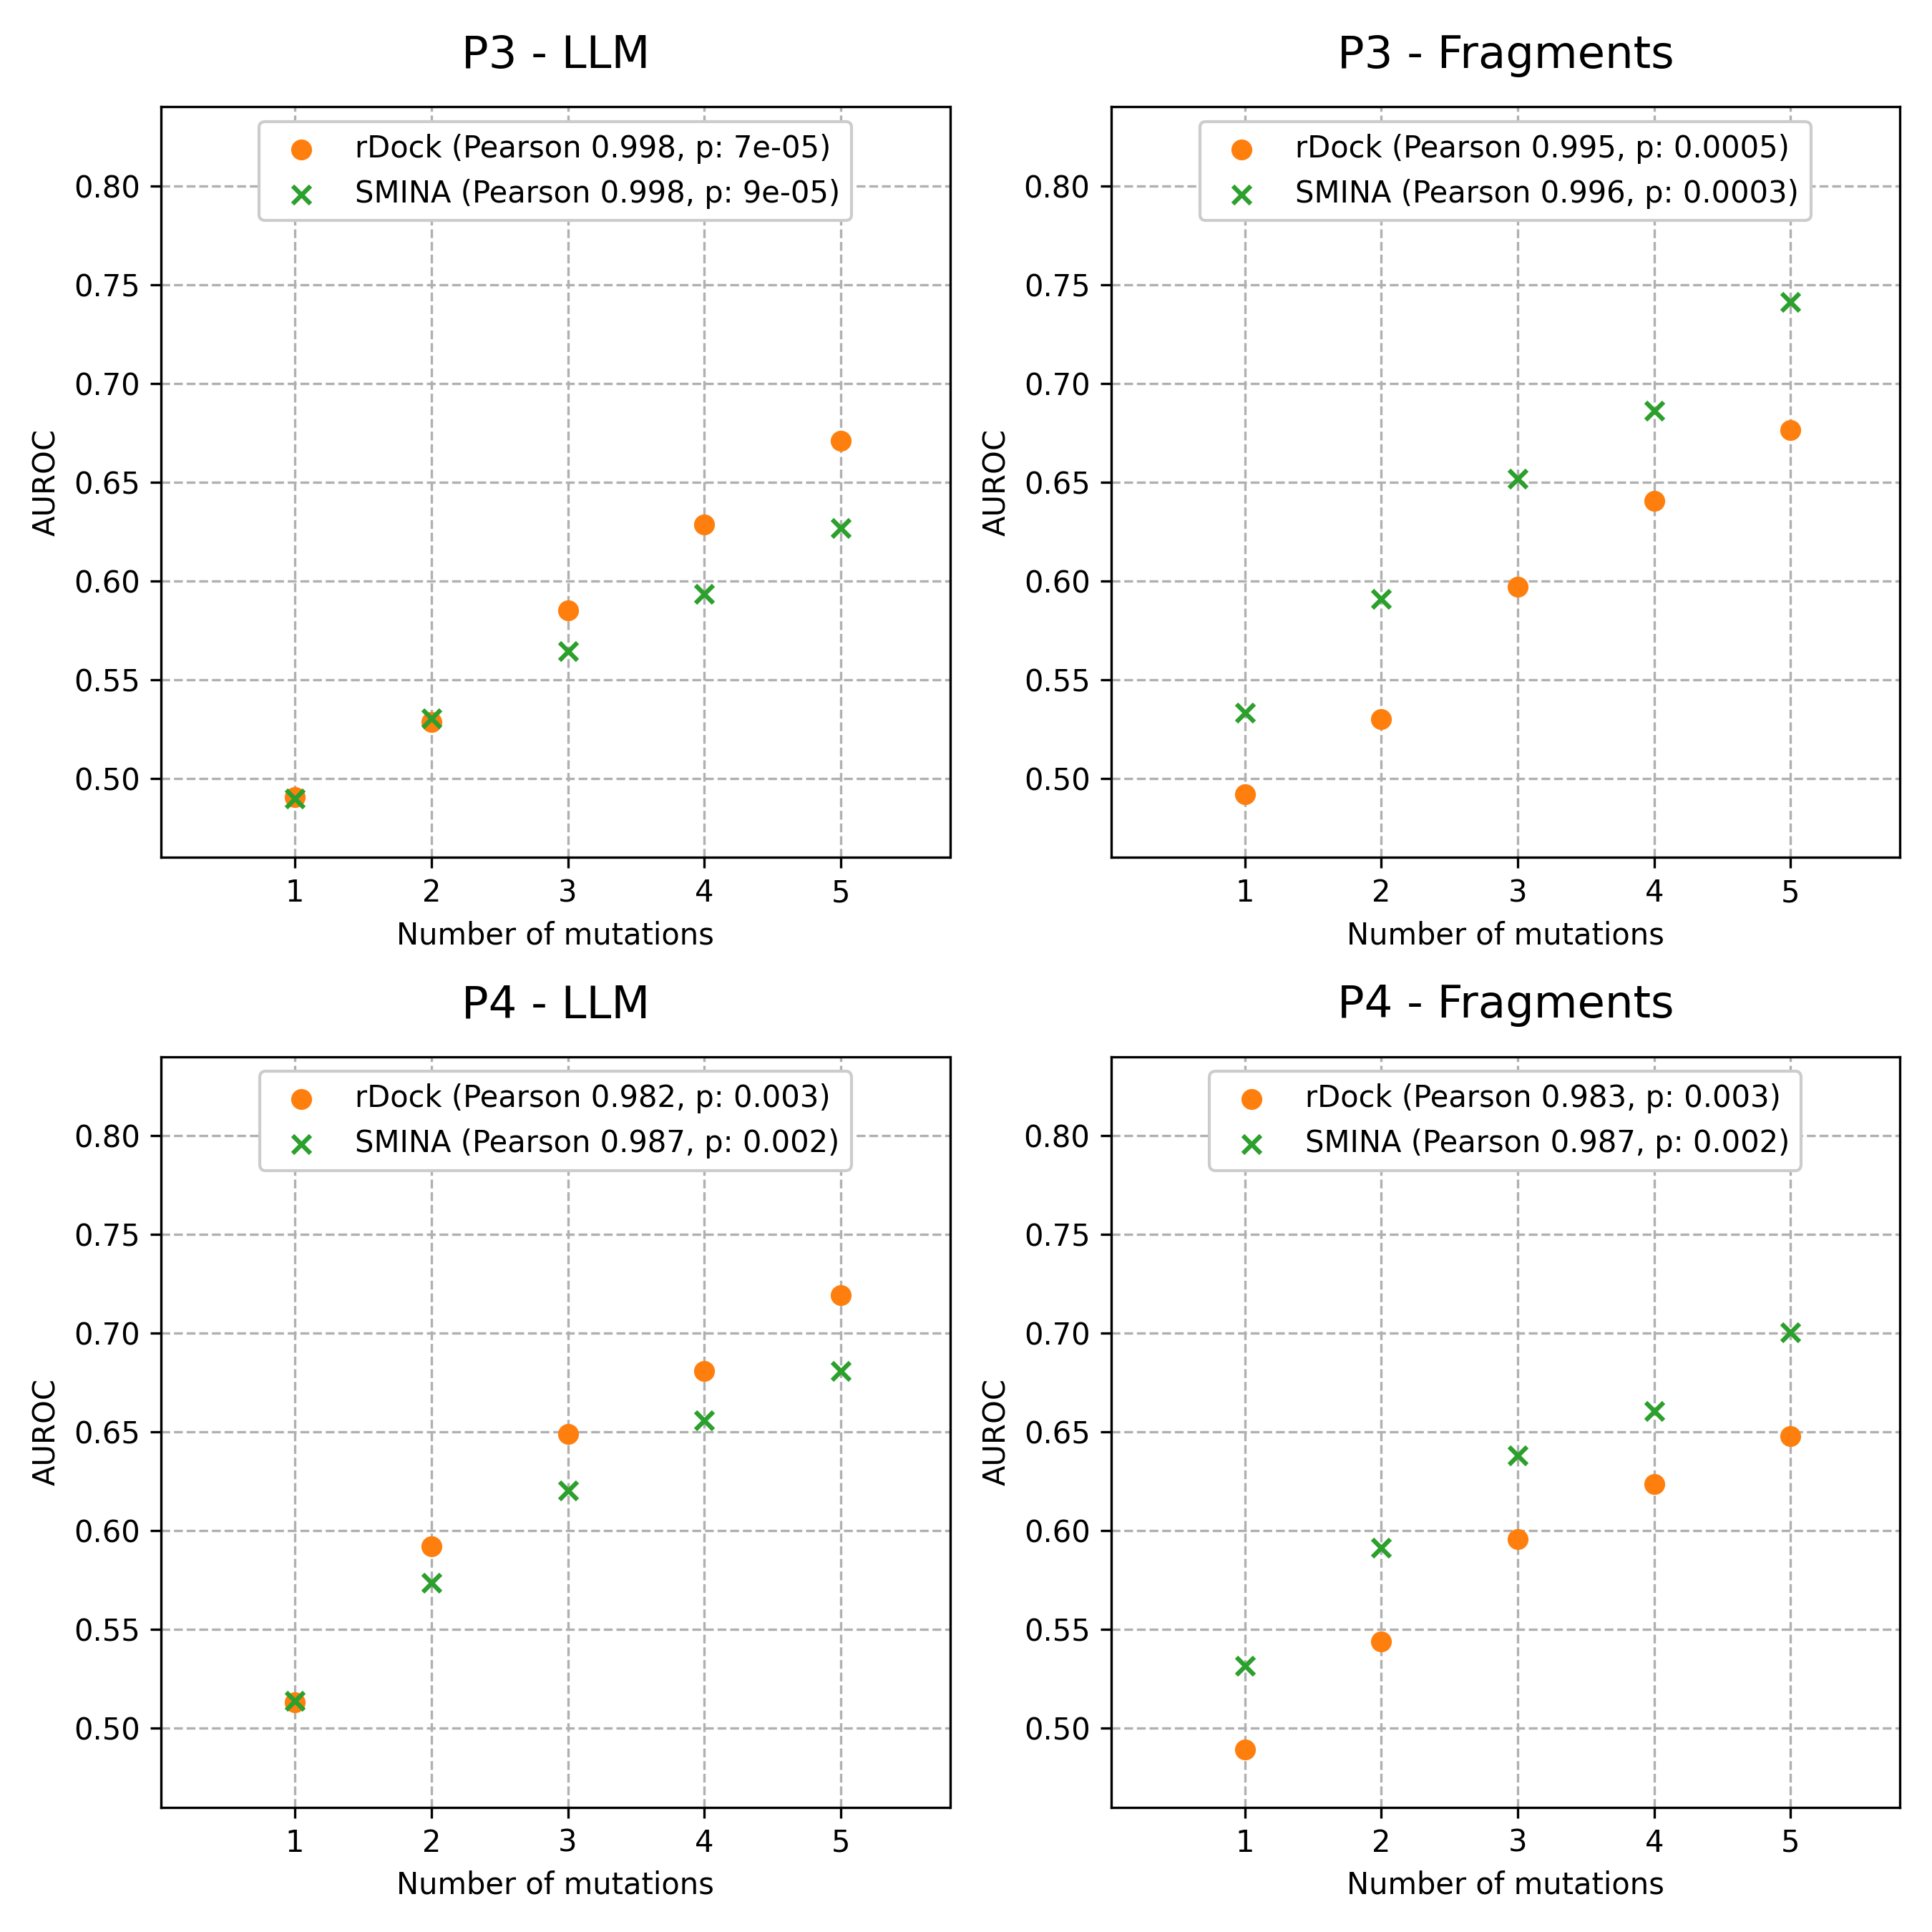
\includegraphics[width=0.8\linewidth]{figures/PocketVec/Supplementary/FigS9.png}
  \caption{
  Correlation between the AUROC (y-axis) and the number of artificial mutations (x-axis) in pocket-lining residues leading to changes in physicochemical properties (ProSPECCTs P3) and both physicochemical and shape properties (ProSPECCTs P4). Each subplot corresponds to a specific ProSPECCTs dataset (P3, P4) and collection of compounds (128 LLM and 128 fragments). Dot color and marker indicate the used docking method (rDock for rigid docking and SMINA for flexible docking). In the legend, the corresponding Pearson’s Correlation Coefficients are reported. 
  }
  \label{FigS9}
\end{figure}

\begin{figure}[htbp]
  \centering
  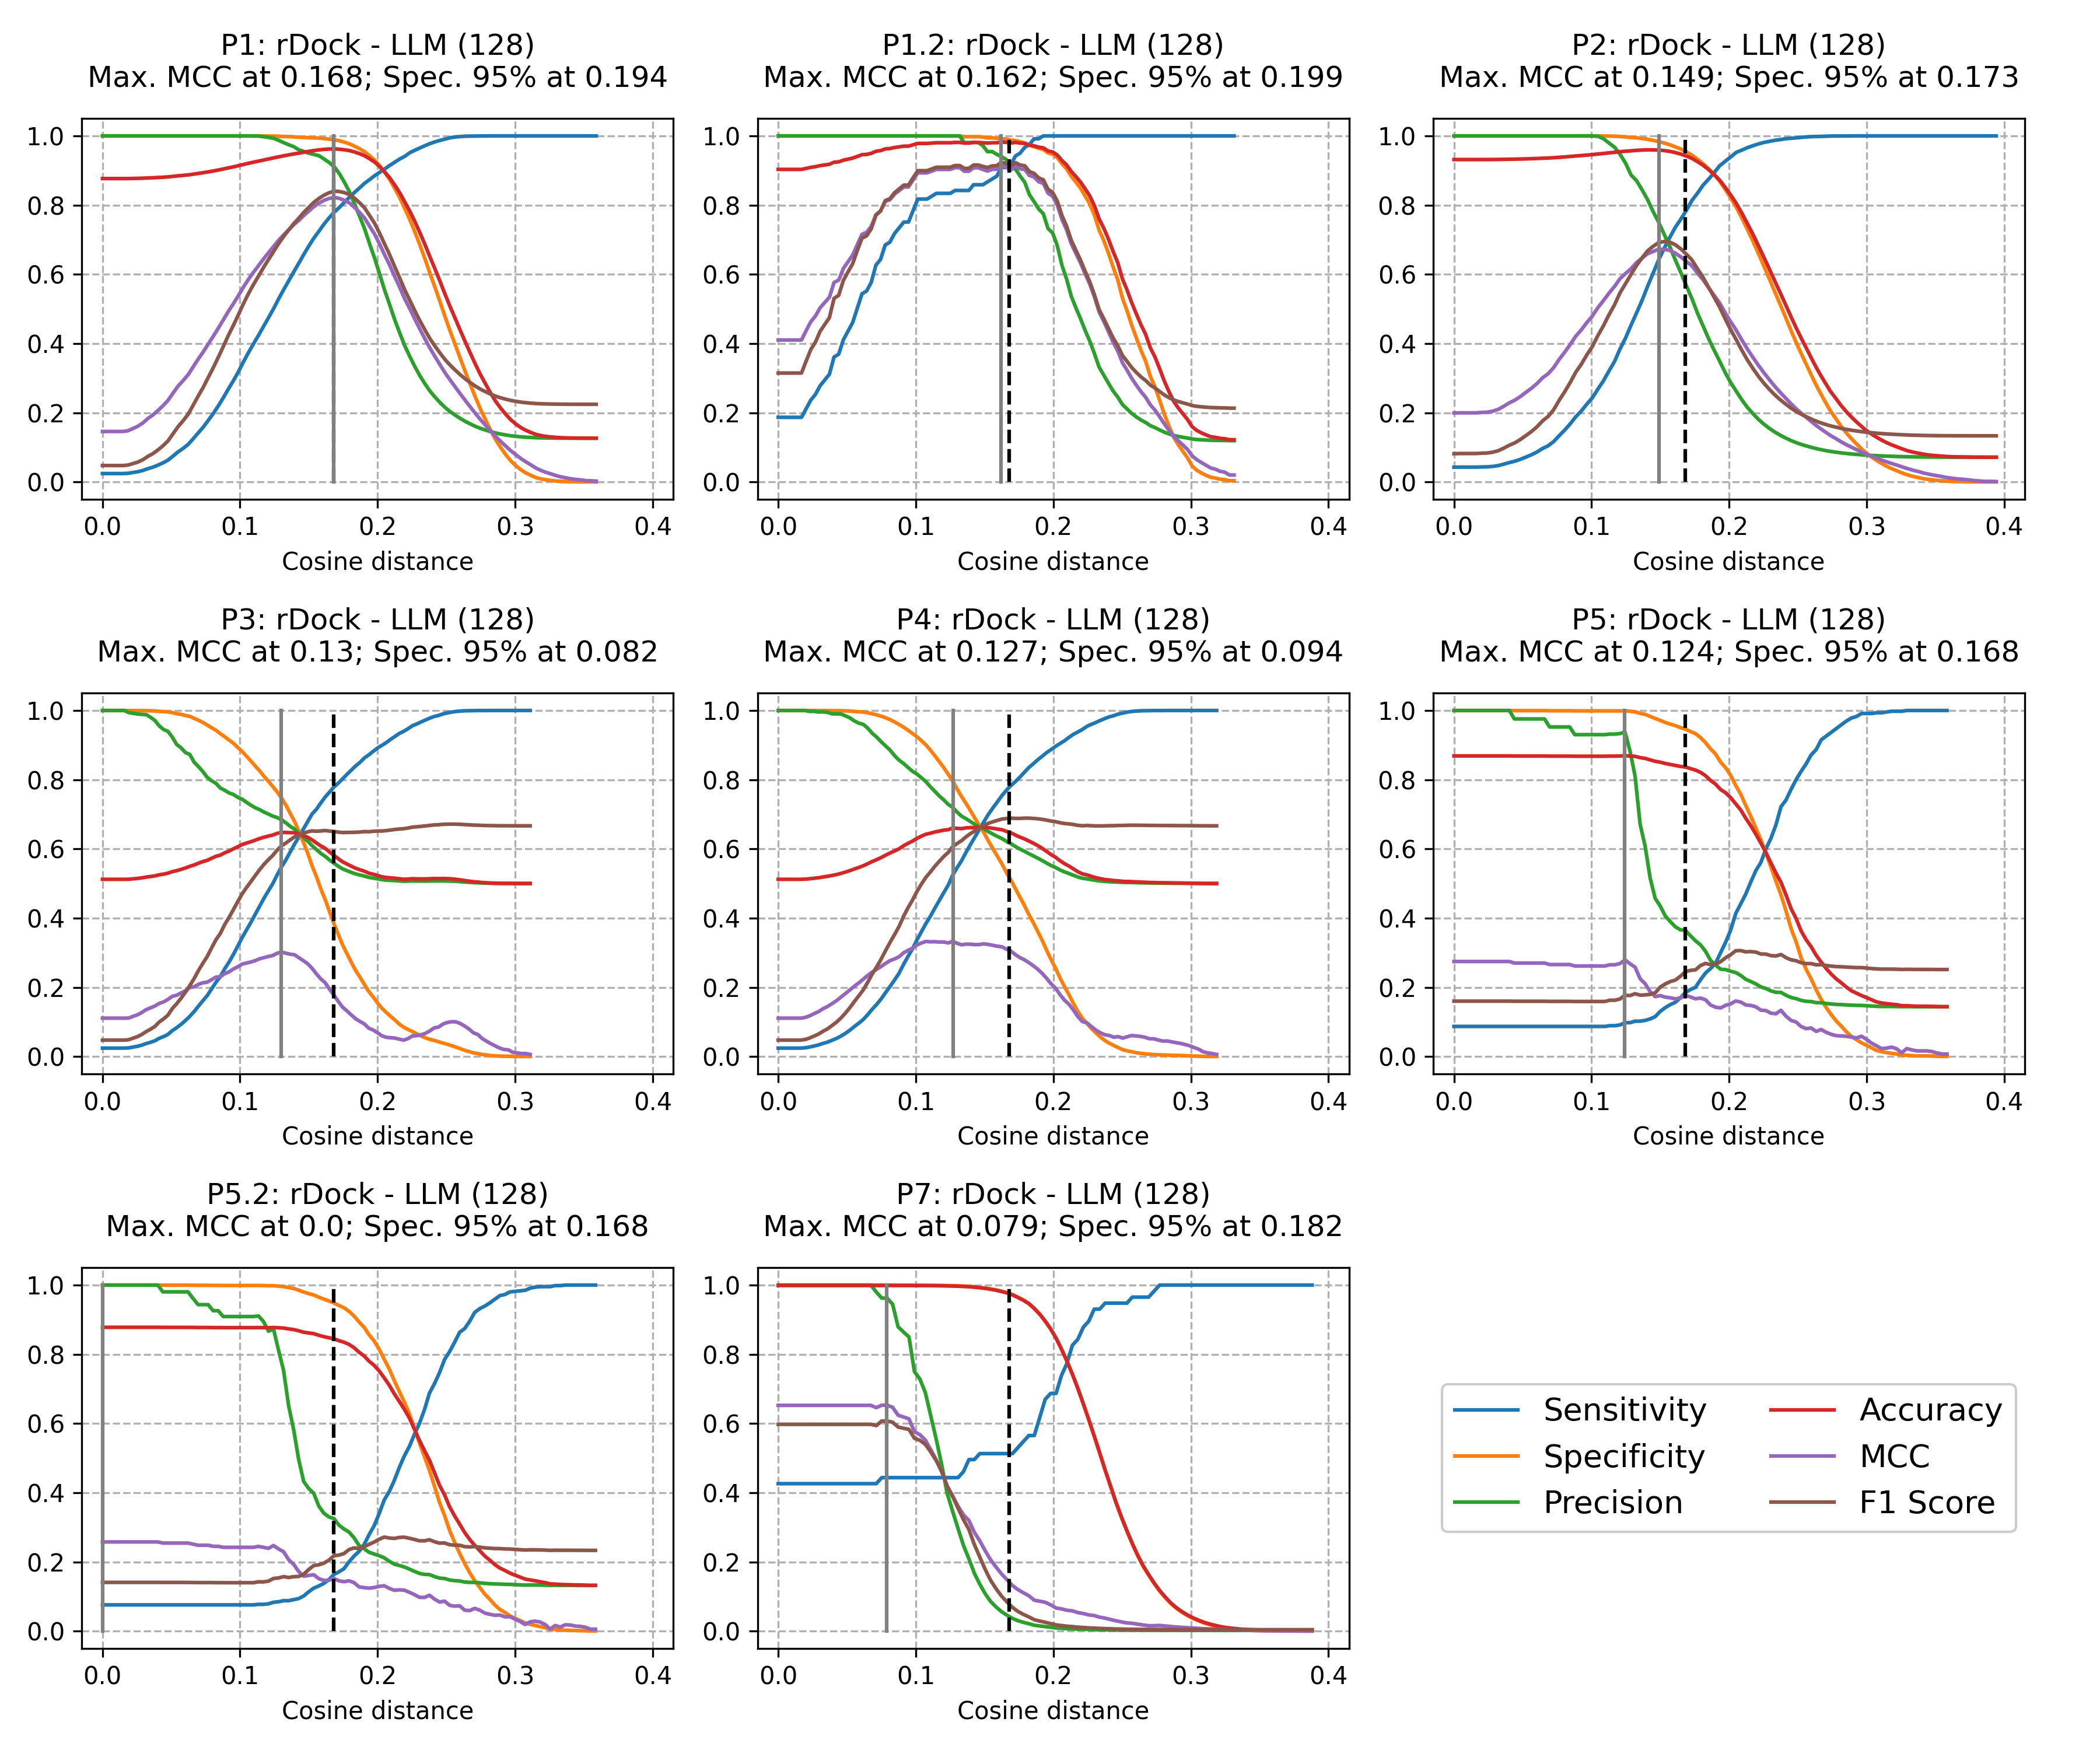
\includegraphics[width=\linewidth]{figures/PocketVec/Supplementary/ProSPECCTs_metrics_evolution.png}
  \caption{
  For each ProSPECCTs dataset, evolution (y-axis) of the Sensitivity (blue), Specificity (orange), Precision (green), Accuracy (red), MCC (purple) and F1 Score (brown) at different distance threshold values (x-axis, cosine distance). The vertical gray thin line represents the cosine distance maximizing the MCC in each ProSPECCTs dataset. The vertical dashed black line represents the cosine distance maximizing the MCC in ProSPECCTs P1 (0.17), which corresponds to the general guideline for classifying a pocket pair of interest as either similar or dissimilar.
  }
  \label{ProSPECCTs_metrics_evolution}
\end{figure}



% \begin{figure}[htbp]
%   \centering
%   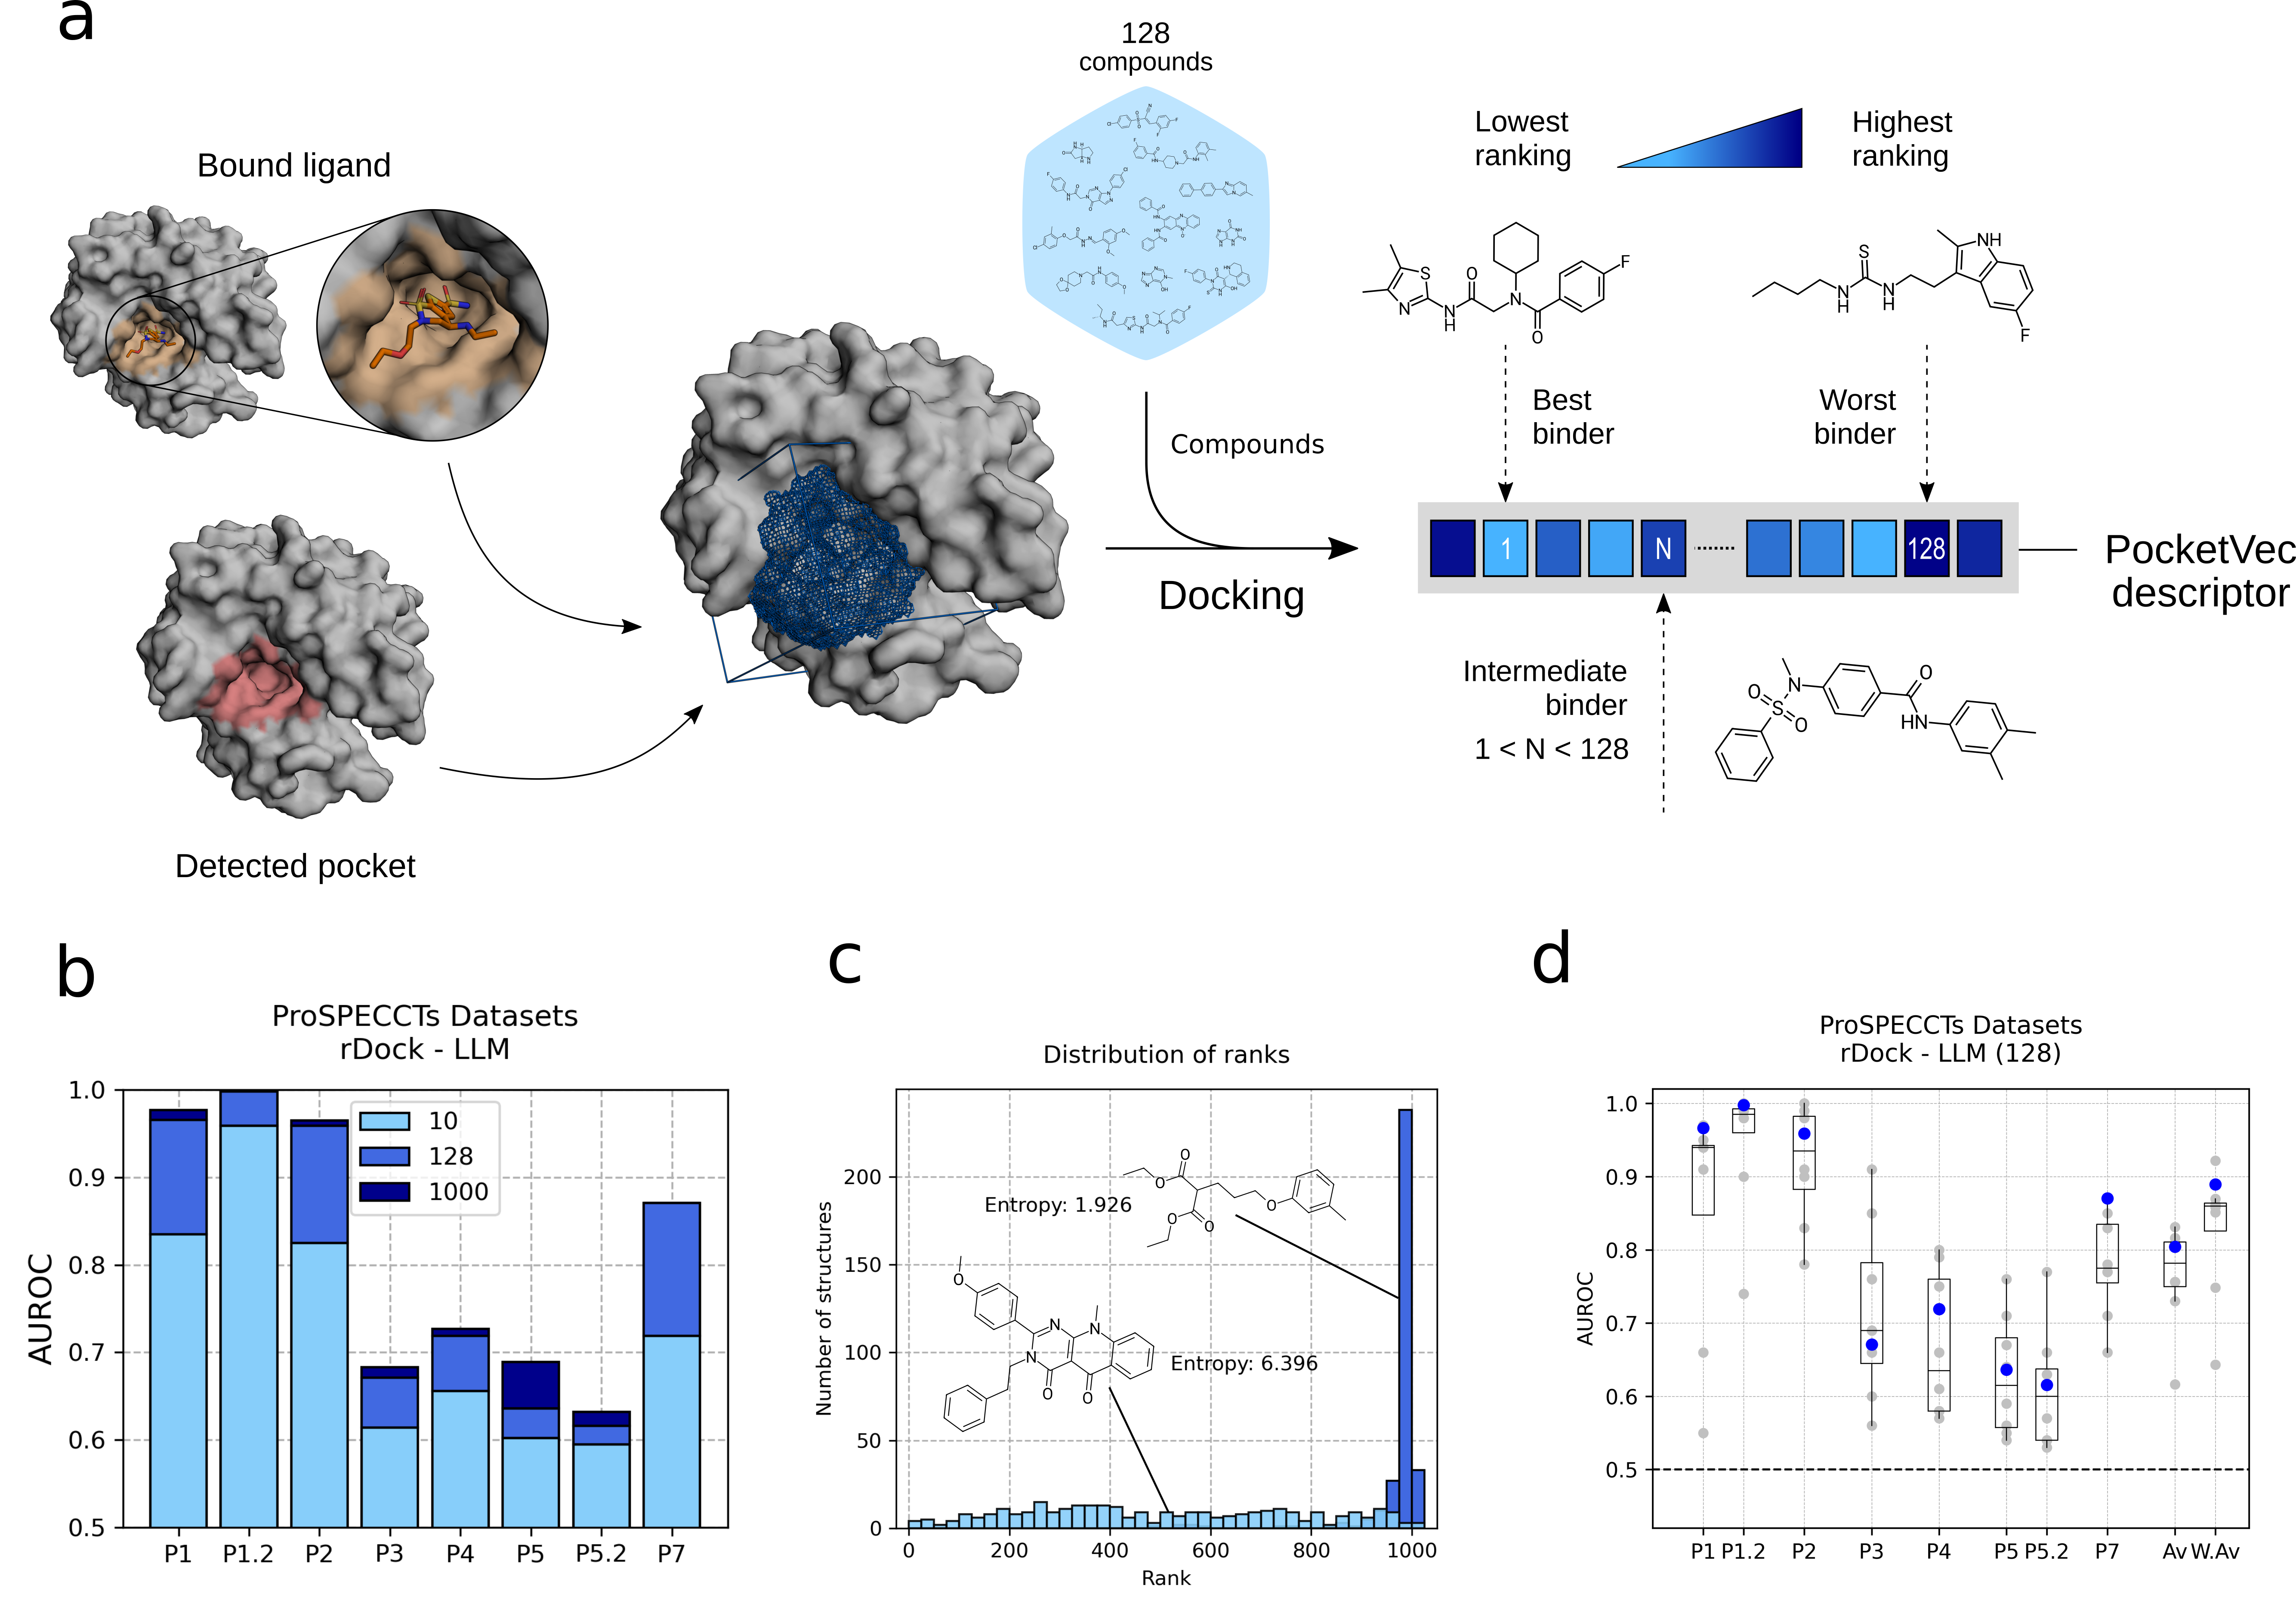
\includegraphics[width=\linewidth]{figures/PocketVec/Main/Fig1.png}
%   \caption{
  
%   }
%   \label{Fig1}
% \end{figure}




%%%%%%%%%%%%%%%%%%%%
%%%%  TABLES  %%%%%%
%%%%%%%%%%%%%%%%%%%%

\newpage

% Define a new column type for tabularx that allows line breaks
\newcolumntype{L}[1]{>{\raggedright\arraybackslash}p{#1}}

% Importing and displaying the CSV file as a table
\csvreader[
    longtable=|L{1.8cm}|L{1.25cm}|L{1.25cm}|L{1.25cm}|L{1.25cm}|L{1.25cm}|L{1.25cm}|L{1.25cm}|L{1.25cm}|L{1.25cm}|L{1.25cm}|L{1.25cm}|,  % Adjust the widths as needed
    table head=\caption{Bla bla bla}\label{TableS1} \\\toprule & \textbf{D1} & \textbf{D1.2} & \textbf{D2} & \textbf{D3} & \textbf{D4} & \textbf{D5} & \textbf{D5.2} & \textbf{D7} & \textbf{Av} & \textbf{W. Av.} \\\midrule\endfirsthead
    \toprule & \textbf{D1} & \textbf{D1.2} & \textbf{D2} & \textbf{D3} & \textbf{D4} & \textbf{D5} & \textbf{D5.2} & \textbf{D7} & \textbf{Av} & \textbf{W. Av.} \\\midrule\endhead
    \bottomrule\endfoot,
    before reading={\catcode`\#=12}, % Handle special characters
    late after line=\\\midrule
]{figures/PocketVec/Supplementary/TableS1.csv}{} % Path to your CSV file
{\csvcoli & \csvcolii & \csvcoliii & \csvcoliv & \csvcolv & \csvcolvi & \csvcolvii & \csvcolviii & \csvcolix & \csvcolx & \csvcolxi}






